\chapter{Конструкторская часть}

В данной главе представлены требования к разрабатываемому программному обеспечению, а также приведены схемы алгоритмов.

\section{Требования к программе}

Для разрабатываемой программы определены следующие задачи.
\begin{enumerate}
	\item Реализовать интерфейс выбора операций для пользователя.
	\item Обеспечить возможность работы программы в двух режимах: одиночное выполнение и массовое измерение времени выполнения.
	\item В рамках режима одиночного запуска необходимо предусмотреть:
	\begin{itemize}
		\item ввод последовательности, оканчивающейся нулём;
		\item проверку корректности введённых данных.
	\end{itemize}
	\item Для режима массового измерения времени требуется фиксировать затраченное процессорное время и выводить результаты в табличном виде.
\end{enumerate}

\section{Разработка алгоритмов}

На рисунке~\ref{recursive} представлена схема рекурсивного алгоритма вывода элементов последовательности с нечётными номерами. Сам алгоритм называется \texttt{recursive\_print}.

\begin{figure}[h!]
	\centering
	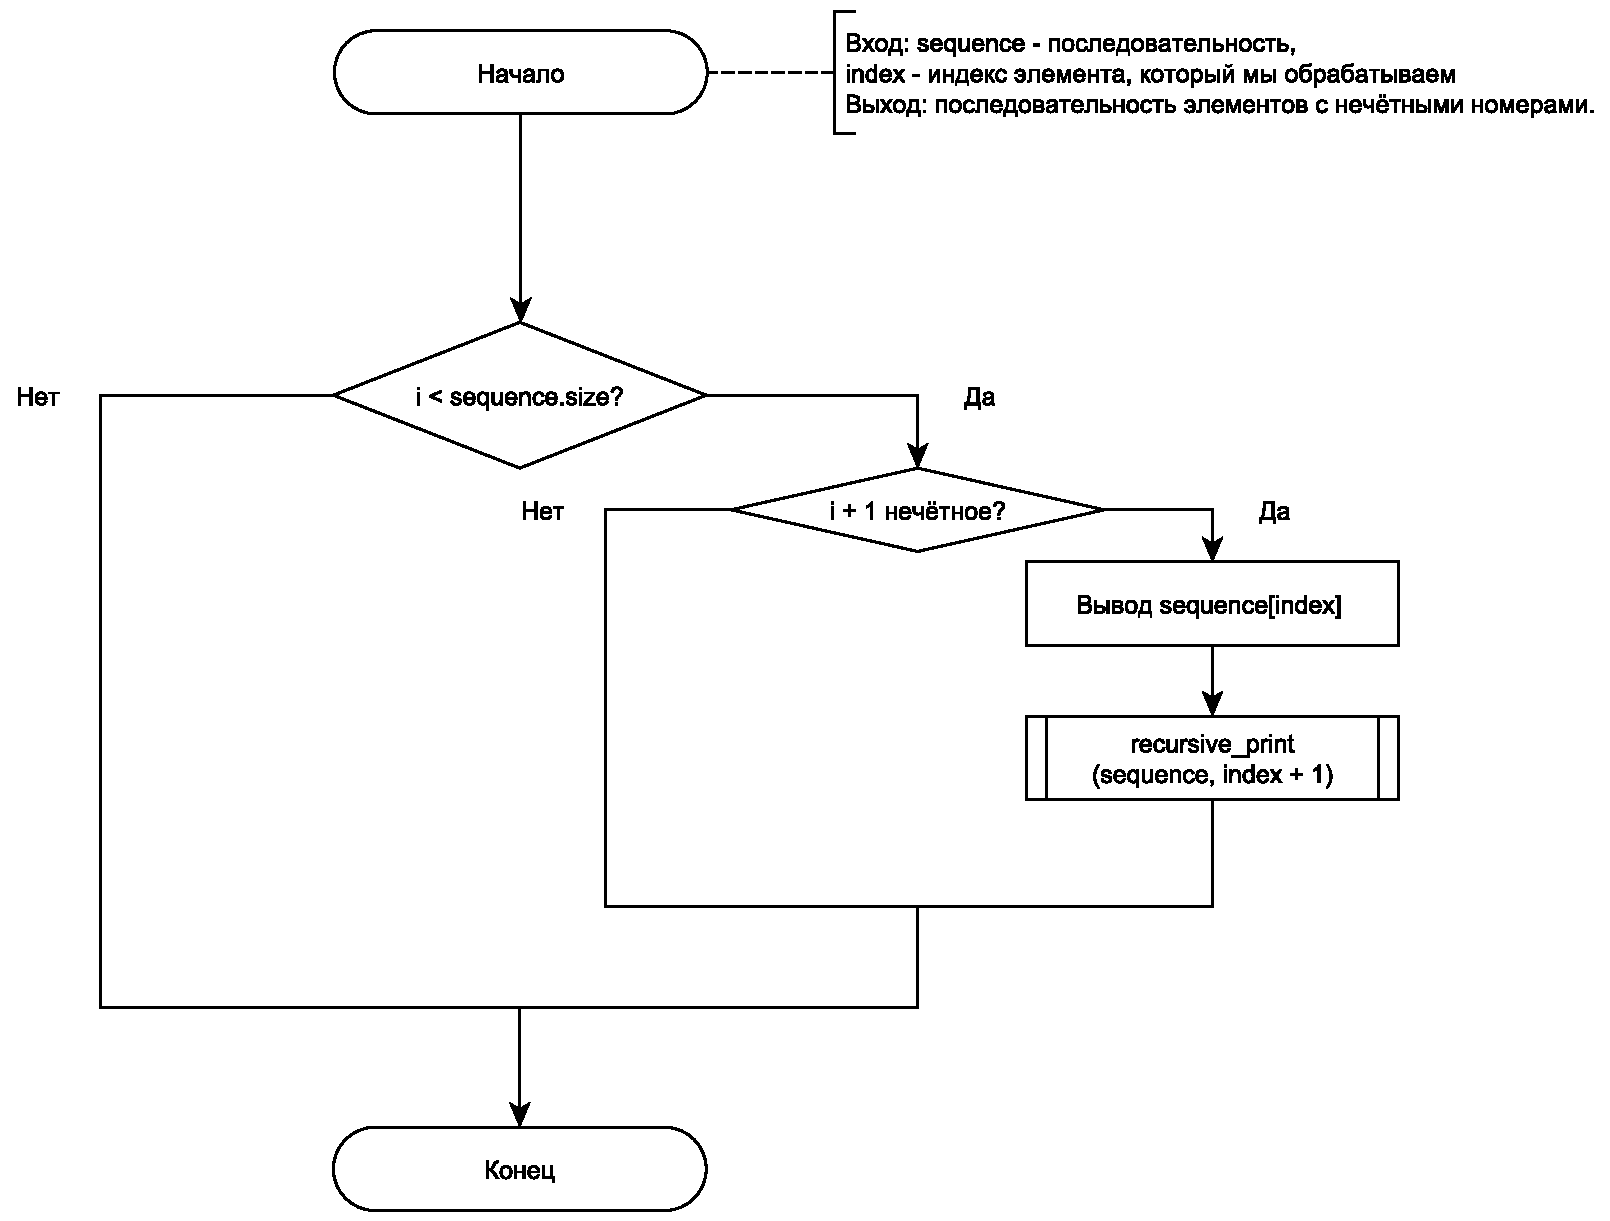
\includegraphics[width=0.9\textwidth, height=0.9\textheight, keepaspectratio]{images/recursive_scheme}
	\caption{Схема рекурсивного алгоритма вывода элементов последовательности с нечётными номерами}
	\label{recursive}
\end{figure}
\clearpage

На рисунке~\ref{iteration} представлена схема итеративного алгоритма вывода элементов последовательности с нечётными номерами.

\begin{figure}[h!]
	\centering
	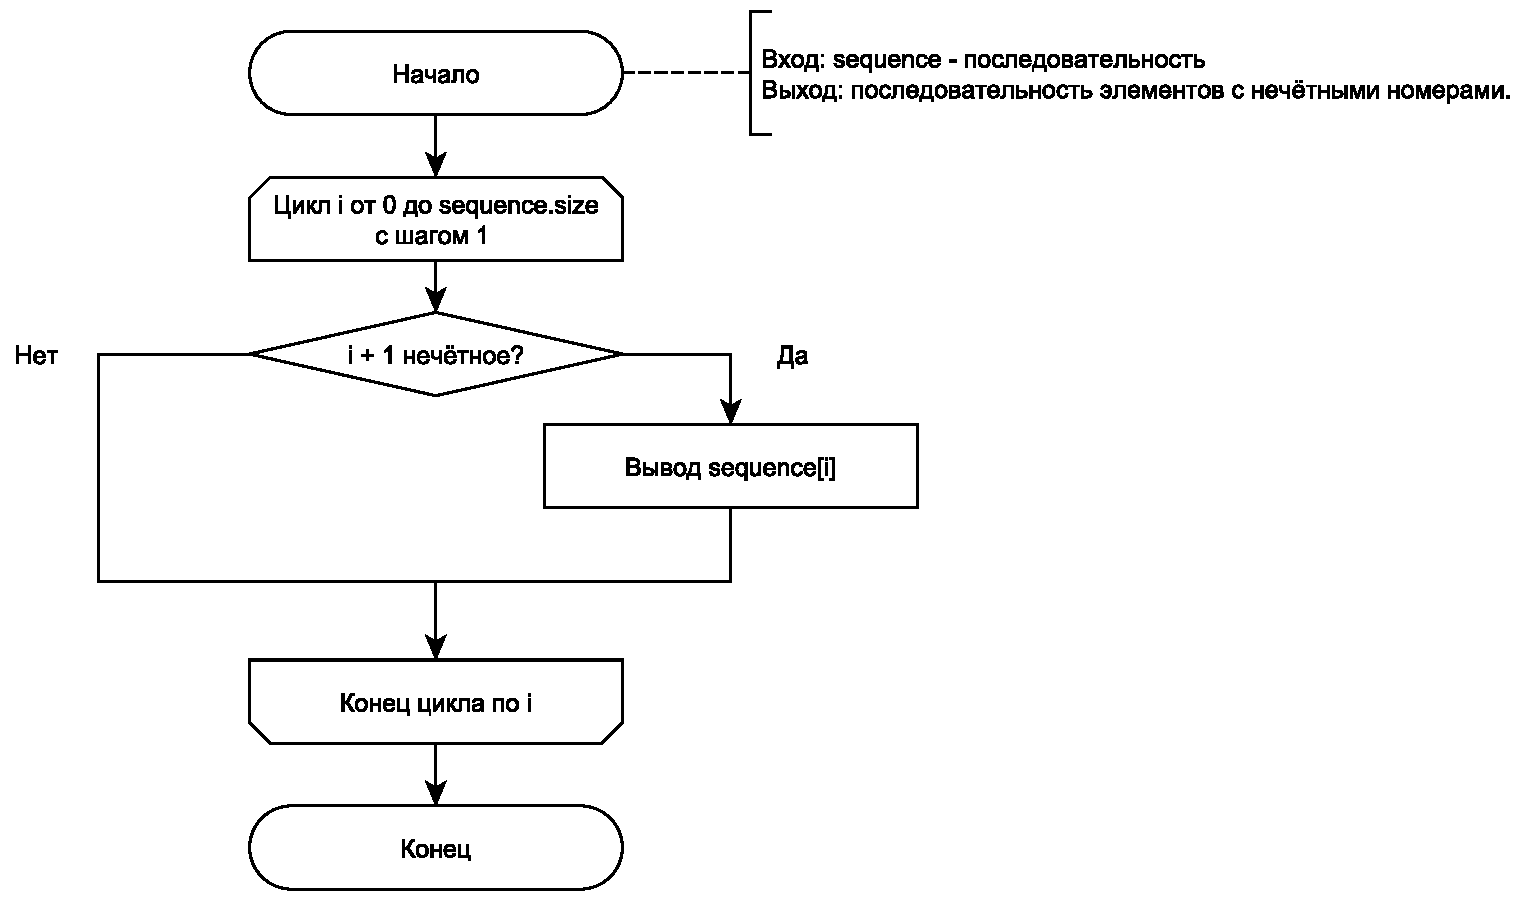
\includegraphics[width=0.9\textwidth, height=0.9\textheight, keepaspectratio]{images/iteration}
	\caption{Схема итеративного алгоритма вывода элементов последовательности с нечётными номерами}
	\label{iteration}
\end{figure}

\section*{Вывод}

В данной главе были сформулированы требования к разрабатываемому программному обеспечению, приведены схемы алгоритмов вывода элементов последовательности с нечётными номерами.  

